% AI Fairness Dashboard — Formal Report
% Compile: pdflatex report.tex  (run twice for references)
\documentclass[11pt,a4paper]{article}

\usepackage[utf8]{inputenc}
\usepackage[T1]{fontenc}
\usepackage{lmodern}
\usepackage[margin=1in]{geometry}
\usepackage{graphicx}
\usepackage{booktabs}
\usepackage{array}
\usepackage{float}
\usepackage{hyperref}
\usepackage{amsmath}
\usepackage{enumitem}
\usepackage{caption}
\usepackage{subcaption}
\usepackage{xcolor}
\usepackage{tabularx}
\usepackage{multirow}

\hypersetup{
    colorlinks=true,
    linkcolor=blue!70!black,
    citecolor=blue!70!black,
    urlcolor=blue!70!black,
}

\graphicspath{{../artifacts/visualizations/}}

\title{%
  \textbf{Fairness Audit Benchmark for Lending Datasets:}\\[4pt]
  \large An Evaluation Protocol for OpenAI-Based, Remediation-Ready Audits
}
\author{
  NeurIPS 2026 Evaluations \& Datasets Artifact
}
\date{\today}

\begin{document}
\maketitle

% ===================================================================
\begin{abstract}
Algorithmic decision-making in lending carries significant fairness risks:
models trained on historical data can perpetuate and amplify biases along
demographic lines. This report frames the project as a NeurIPS Evaluations
\& Datasets style artifact: an evaluation protocol and benchmark for testing
whether LLM-based fairness auditors produce stable, statistically grounded,
remediation-ready audits on lending datasets. We apply a deterministic
fairness pipeline to the UCI German Credit dataset and the U.S.\ Home
Mortgage Disclosure Act (HMDA) dataset for Georgia, then evaluate an OpenAI
LLM auditor that receives Python-computed metric context and is asked to
produce severity labels, root-cause narratives, and mitigation plans. We do
not claim that the LLM independently recomputes fairness metrics; instead,
we evaluate whether it reasons reliably from fixed quantitative evidence.
Results show moderate disparities across several protected attributes and
highlight recurring risks: small subgroup instability, proxy features,
historical label bias, and API/model-version nondeterminism.
\end{abstract}

% ===================================================================
\section{Introduction}

Automated lending decisions---credit scoring, mortgage approvals, loan
pricing---increasingly rely on machine learning models. While these models
improve efficiency, they risk encoding historical biases present in
training data, leading to disparate outcomes for protected groups defined
by sex, age, race, or national origin.

Regulatory frameworks such as the U.S.\ Equal Credit Opportunity Act (ECOA)
and the EU AI Act mandate that lending models be audited for discriminatory
impact. However, detecting bias requires more than a single metric: it
demands multi-dimensional quantitative measurement, qualitative root-cause
analysis, and independent validation.

This artifact makes three contributions:
\begin{enumerate}[nosep]
  \item A \textbf{reproducible fairness pipeline} that preprocesses data,
        trains classifiers, computes five AIF360-based metrics, and generates
        structured reports for each protected attribute.
  \item A \textbf{deterministic qualitative analysis engine} that diagnoses
        data imbalance, detects proxy features, maps root causes, and
        recommends specific mitigations.
  \item An \textbf{OpenAI LLM benchmark} that tests whether a model can turn
        fixed Python-computed metric evidence into stable, statistically
        cautious, remediation-ready fairness audits. Gemini results are kept
        only as secondary legacy comparisons.
\end{enumerate}

% ===================================================================
\section{Background and Related Work}

\subsection{Fairness Metrics}

We adopt five widely-used group fairness metrics. Let $\hat{Y}$ denote
predictions, $Y$ ground truth, and $A$ the protected attribute with
privileged group $a_p$ and unprivileged group $a_u$.

\begin{itemize}[nosep]
  \item \textbf{Disparate Impact (DI)}: ratio of selection rates.
        $\text{DI} = P(\hat{Y}{=}1 \mid A{=}a_u)\;/\;P(\hat{Y}{=}1 \mid A{=}a_p)$.
        Values below 0.8 indicate adverse impact (four-fifths rule).
  \item \textbf{Demographic Parity Difference (DPD)}: difference of selection
        rates, $P(\hat{Y}{=}1 \mid A{=}a_u) - P(\hat{Y}{=}1 \mid A{=}a_p)$.
  \item \textbf{Equal Opportunity Difference (EOD)}: difference of true
        positive rates,
        $\text{TPR}(a_u) - \text{TPR}(a_p)$.
  \item \textbf{Average Odds Difference (AOD)}:
        $\frac{1}{2}[(\text{FPR}(a_u){-}\text{FPR}(a_p)) +
        (\text{TPR}(a_u){-}\text{TPR}(a_p))]$.
  \item \textbf{Theil Index}: an entropy-based inequality measure over
        predicted benefits.
\end{itemize}

\subsection{Fairness Toolkits}

\textbf{AIF360}~\cite{aif360} (IBM) provides dataset wrappers, metric
classes, and pre-/in-/post-processing mitigation algorithms.
\textbf{Fairlearn}~\cite{fairlearn} (Microsoft) offers constraint-based
reduction algorithms (\texttt{ExponentiatedGradient}, \texttt{GridSearch})
and the \texttt{ThresholdOptimizer} post-processor. Our deterministic
pipeline uses AIF360 metric definitions, while the LLM benchmark is
constrained to fairlearn.

\subsection{LLMs as Fairness Auditors}

Recent work has explored using large language models to interpret model
behavior and generate natural-language explanations of bias. In this artifact
we treat the deterministic Python pipeline as the source of record for
fairness metrics. The OpenAI benchmark receives the resulting metric context,
group counts, severity thresholds, and supporting literature context; its
task is to produce qualitative analysis that is grounded in those values.
This design avoids overclaiming that an LLM is a reliable calculator and
instead evaluates the more practical question of whether it can produce
remediation-ready audit narratives from fixed evidence.

% ===================================================================
\section{Datasets}

\subsection{German Credit Dataset}

The UCI Statlog German Credit dataset contains 1{,}000 consumer credit
records. We merge the original Statlog encoding with a Kaggle-hosted
version to obtain human-readable feature names. Protected attributes are
derived as follows:
\begin{itemize}[nosep]
  \item \textbf{Sex}: extracted from personal status codes (Attribute~9).
  \item \textbf{AgeGroup}: binarized at 40 ($<$40 $\rightarrow$ \texttt{under\_40}, $\geq$40 $\rightarrow$ \texttt{40\_plus}).
  \item \textbf{Foreign Worker}: extracted from Attribute~20 (A201/A202 encoding).
\end{itemize}
The target variable is credit reliability (1~=~good, 0~=~bad). An 80/20
train-test split yields 200 test records for fairness evaluation.

\subsection{HMDA Mortgage Lending (Georgia)}

The Home Mortgage Disclosure Act requires U.S.\ lenders to report
application-level data. We download 2022 Georgia records from the
CFPB Data Browser API, filtering to originated and denied applications.
After cleaning and sampling, the dataset contains 6{,}525 records.
Protected attributes:
\begin{itemize}[nosep]
  \item \textbf{Race}: White, Black, Asian, American Indian, Pacific Islander, Multiracial.
  \item \textbf{Sex}: Male, Female.
  \item \textbf{Age Group}: young ($<$35), mid (35--54), senior ($\geq$55).
\end{itemize}
The target is loan approval (1~=~originated, 0~=~denied). A 2{,}196-record
test set is used for evaluation.

\begin{table}[H]
\centering
\caption{Dataset summary.}
\label{tab:datasets}
\begin{tabular}{lcccccc}
\toprule
\textbf{Dataset} & \textbf{Records} & \textbf{Test Set} & \textbf{Features} & \textbf{Protected Attrs} & \textbf{Target} & \textbf{\% Favorable} \\
\midrule
German Credit    & 1{,}000 & 200   & 10 & 3 (Sex, Age, Foreign) & Credit reliability & 70\% \\
HMDA (Georgia)   & 6{,}525 & 2{,}196 & 8  & 3 (Race, Sex, Age)    & Loan approval      & 72\% \\
\bottomrule
\end{tabular}
\end{table}

% ===================================================================
\section{Methodology}

\subsection{Pipeline Architecture}

All analysis is orchestrated by a central pipeline (\texttt{run\_pipeline.py})
that executes six sequential steps per dataset:

\begin{center}
\texttt{clean} $\rightarrow$ \texttt{train} $\rightarrow$
\texttt{fairness} $\rightarrow$ \texttt{qualitative} $\rightarrow$
\texttt{llm\_benchmark} $\rightarrow$ \texttt{visualize}
\end{center}

A consolidation step then merges per-dataset results into cross-dataset
reports and comparison visualizations. The pipeline supports selective
execution (e.g., rerunning only the LLM benchmark step).

\subsection{Model Training}

For each dataset, we train two classifiers---Logistic Regression and
Random Forest---using scikit-learn. Continuous features are standardized
(\texttt{StandardScaler}), categorical features are label-encoded, and
missing values are imputed with the mode. We use an 80/20 stratified
train-test split. Predictions on the test set are exported with original
protected attribute labels preserved for downstream fairness analysis.

\subsection{Fairness Metric Computation}

For each protected attribute, we define the privileged group based on
domain knowledge (Table~\ref{tab:priv}). Five metrics are computed:
DI, DPD, EOD, AOD, and Theil Index. A bias flag is raised when
DI~$<$~0.8. Results are exported to CSV and Markdown reports.

\begin{table}[H]
\centering
\caption{Privileged group definitions.}
\label{tab:priv}
\begin{tabular}{llll}
\toprule
\textbf{Dataset} & \textbf{Attribute} & \textbf{Privileged} & \textbf{Rationale} \\
\midrule
German Credit & Sex              & Male     & Historically advantaged in credit \\
              & AgeGroup         & 40+      & Longer credit history \\
              & Foreign Worker   & Non-foreign (0) & Domestic applicants favored \\
\midrule
HMDA          & Race             & White    & Majority, historically favored \\
              & Sex              & Male     & Historically advantaged \\
              & Age Group        & Mid (35--54) & Peak earning years \\
\bottomrule
\end{tabular}
\end{table}

\subsection{Qualitative Analysis Engine}

Our deterministic qualitative module (\texttt{qualitative\_analysis.py})
performs four analyses per protected attribute:

\begin{enumerate}[nosep]
  \item \textbf{Per-group breakdown}: selection rates, TPR, FPR, and base
        rates for every subgroup.
  \item \textbf{Data imbalance diagnosis}: flags group size ratios
        $>$3$\times$, groups with $<$30 records, and base-rate disparities
        $>$15\%.
  \item \textbf{Proxy feature detection}: computes point-biserial
        correlation (binary attributes) or eta-squared (multi-class) between
        each numeric feature and the protected attribute, flagging
        correlations $\geq$0.15.
  \item \textbf{Root-cause mapping}: a rule engine maps metric patterns
        (e.g., $|\text{EOD}| > 0.05$) and detected proxies to specific root
        causes and AIF360 mitigation algorithms.
\end{enumerate}

Each attribute receives a severity classification: \textsc{Critical}
(DI~$<$~0.72), \textsc{High} (0.72--0.80), \textsc{Moderate} (0.80--0.95),
or \textsc{Low} ($\geq$0.95).

\subsection{OpenAI LLM Benchmark}

The primary LLM benchmark uses OpenAI. Python first constructs a metric
context from the predictions CSV, deterministic fairness metrics, group
breakdowns, severity thresholds, root-cause candidates, mitigation
candidates, and Semantic Scholar evidence when available. The prompt then
instructs OpenAI to:
\begin{itemize}[nosep]
  \item Do \textbf{not} recompute fairness metrics.
  \item Interpret the Python-computed DI, DPD, EOD, AOD, Theil, group counts,
        and severity context.
  \item Produce qualitative analysis: what is wrong, why, and how to fix it
        using AIF360/Fairlearn mitigation concepts.
  \item Return structured JSON for programmatic comparison.
\end{itemize}

The benchmark therefore measures metric-grounded reasoning, severity
alignment, mitigation specificity, and research grounding. Gemini outputs
from earlier experiments remain useful as secondary legacy comparisons, but
they are not the primary benchmark story for this artifact.

% ===================================================================
\section{Results}

\subsection{German Credit: Fairness Metrics}

\begin{table}[H]
\centering
\caption{German Credit fairness metrics (our pipeline).}
\label{tab:gc-metrics}
\begin{tabular}{lccccc}
\toprule
\textbf{Attribute} & \textbf{DI} & \textbf{DPD} & \textbf{EOD} & \textbf{AOD} & \textbf{Theil} \\
\midrule
Sex (priv: male)              & 0.8595 & $-$0.1152 & $-$0.0512 & $-$0.1256 & 0.3084 \\
AgeGroup (priv: 40+)          & 0.8212 & $-$0.1586 & $-$0.0513 & $-$0.1649 & 0.3084 \\
Foreign Worker (priv: non-fw)  & 0.9402 & $-$0.0498 & $-$0.0889 & $+$0.2013 & 0.3084 \\
\bottomrule
\end{tabular}
\end{table}

All three attributes fall in the \textsc{Moderate} severity range
(DI between 0.80 and 0.95). Sex and AgeGroup show consistent disadvantage
for the unprivileged group across all metrics. Foreign Worker metrics are
unreliable due to extreme group imbalance (194 vs.\ 6 records).

\begin{figure}[H]
\centering
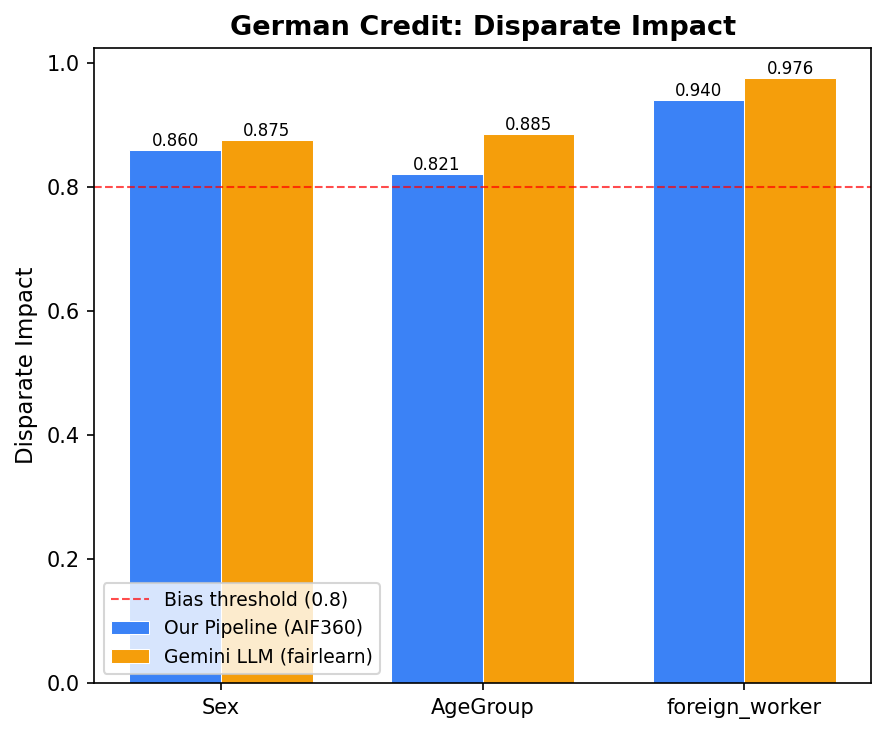
\includegraphics[width=0.85\textwidth]{german_credit_disparate_impact.png}
\caption{German Credit: Disparate Impact by protected attribute
         (pipeline vs.\ LLM).}
\label{fig:gc-di}
\end{figure}

\subsection{HMDA: Fairness Metrics}

\begin{table}[H]
\centering
\caption{HMDA (Georgia) fairness metrics (our pipeline).}
\label{tab:hmda-metrics}
\begin{tabular}{lccccc}
\toprule
\textbf{Attribute} & \textbf{DI} & \textbf{DPD} & \textbf{EOD} & \textbf{AOD} & \textbf{Theil} \\
\midrule
Race (priv: White)     & 0.8956 & $-$0.0776 & $+$0.0025 & $+$0.0117 & 0.4838 \\
Sex (priv: Male)       & 0.9291 & $-$0.0518 & $-$0.0076 & $-$0.0084 & 0.4838 \\
Age Group (priv: mid)  & 1.0138 & $+$0.0097 & $+$0.0008 & $-$0.0150 & 0.4838 \\
\bottomrule
\end{tabular}
\end{table}

Race exhibits \textsc{Moderate} bias (DI~=~0.8956), sex is borderline
\textsc{Moderate} (DI~=~0.9291), and age group is effectively fair
(DI~=~1.0138). The small EOD and AOD values for HMDA suggest the model's
error rates are relatively balanced across groups, with the primary
disparity being in overall selection rates.

\begin{figure}[H]
\centering
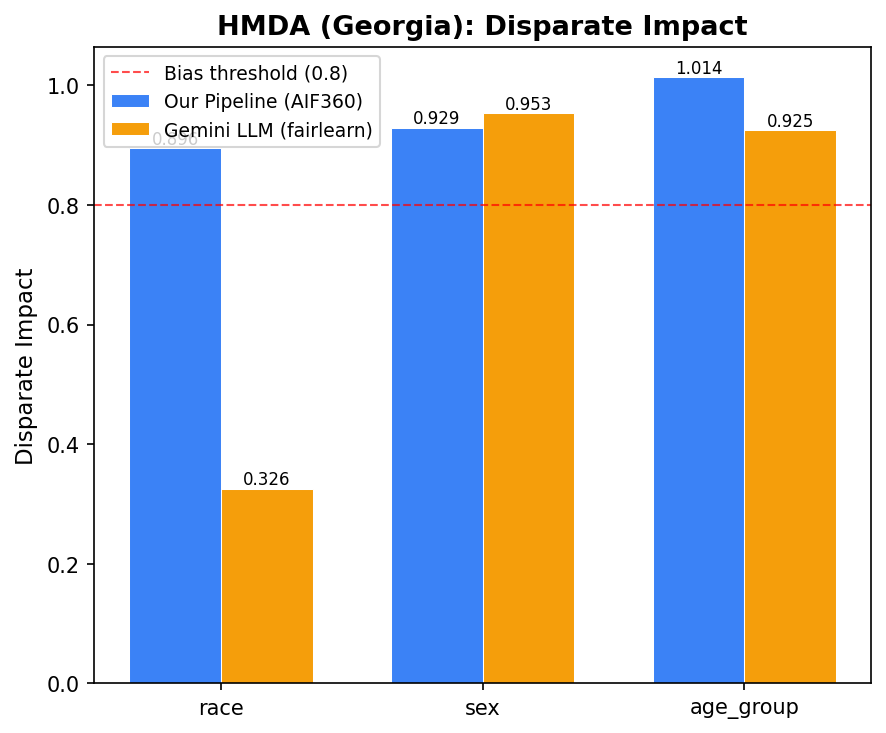
\includegraphics[width=0.85\textwidth]{hmda_disparate_impact.png}
\caption{HMDA: Disparate Impact by protected attribute
         (pipeline vs.\ LLM).}
\label{fig:hmda-di}
\end{figure}

\subsection{Qualitative Findings}

The qualitative engine identified the following root causes:

\paragraph{German Credit.}
\begin{itemize}[nosep]
  \item \textbf{Sex}: Strong proxy feature detected (\texttt{Sex} column,
        $r{=}1.0$); the encoded Sex feature directly leaks into the model.
        Weaker proxies include Housing ($r{=}{-}0.27$) and Age ($r{=}0.22$).
        Root causes: proxy discrimination, unequal opportunity
        (EOD~$=$~$-$0.05), and unequal odds (AOD~$=$~$-$0.13).
  \item \textbf{AgeGroup}: Strong proxy via Age ($r{=}{-}0.84$) and the
        AgeGroup encoding itself. Historical label bias detected: 40+
        borrowers have a 77.5\% favorable base rate vs.\ 65.9\% for under-40.
  \item \textbf{Foreign Worker}: Severe size imbalance (194 vs.\ 6 records,
        32$\times$ ratio). Metrics for the non-foreign group are statistically
        unreliable ($n{=}6$). Root cause: representation bias.
\end{itemize}

\paragraph{HMDA.}
\begin{itemize}[nosep]
  \item \textbf{Race}: Severe size imbalance (White: 1{,}252 vs.\ Pacific
        Islander: 5, a 250$\times$ ratio). Base-rate disparity: Asian
        applicants have 79.8\% favorable outcomes vs.\ Multiracial at 37.5\%
        (gap~$=$~42.3\%). Root causes: historical/label bias and
        representation bias.
  \item \textbf{Sex}: Borderline disparity with no strong root cause
        detected by the rule engine. Recommended: post-processing threshold
        calibration.
  \item \textbf{Age Group}: No significant disparity (DI~$>$~1.0), though
        historical label bias exists in the ground truth.
\end{itemize}

\subsection{OpenAI Benchmark Comparison}

The OpenAI benchmark is evaluated against the deterministic baseline over
fixed refinement cycles. Because OpenAI receives Python-computed metrics, we
do not compare newly computed LLM metric values. Instead, we compare whether
the LLM preserves severity, uses the supplied evidence, and produces
remediation-ready guidance.

\subsubsection{Cycle Scores}

\begin{table}[H]
\centering
\caption{OpenAI qualitative benchmark cycle scores.}
\label{tab:openai-cycles}
\begin{tabular}{lccc}
\toprule
\textbf{Dataset} & \textbf{Cycle 1} & \textbf{Cycle 2} & \textbf{Cycle 3} \\
\midrule
German Credit & 90.0 & 85.0 & 85.0 \\
HMDA Georgia  & 90.0 & 85.0 & 90.0 \\
\bottomrule
\end{tabular}
\end{table}

\subsubsection{Severity Agreement}

\begin{table}[H]
\centering
\caption{Severity classification agreement: deterministic baseline vs.\ OpenAI.}
\label{tab:severity}
\begin{tabular}{llccl}
\toprule
\textbf{Dataset} & \textbf{Attribute} & \textbf{Baseline} & \textbf{OpenAI} & \textbf{Agree?} \\
\midrule
German Credit & Sex              & Moderate & Moderate & Yes \\
              & AgeGroup         & Moderate & Moderate & Yes \\
              & Foreign Worker   & Moderate & Moderate, unstable & Yes \\
\midrule
HMDA          & Race             & Moderate & Moderate & Yes \\
              & Sex              & Moderate & Moderate & Yes \\
              & Age Group        & Low      & Low      & Yes \\
\bottomrule
\end{tabular}
\end{table}

\begin{figure}[H]
\centering
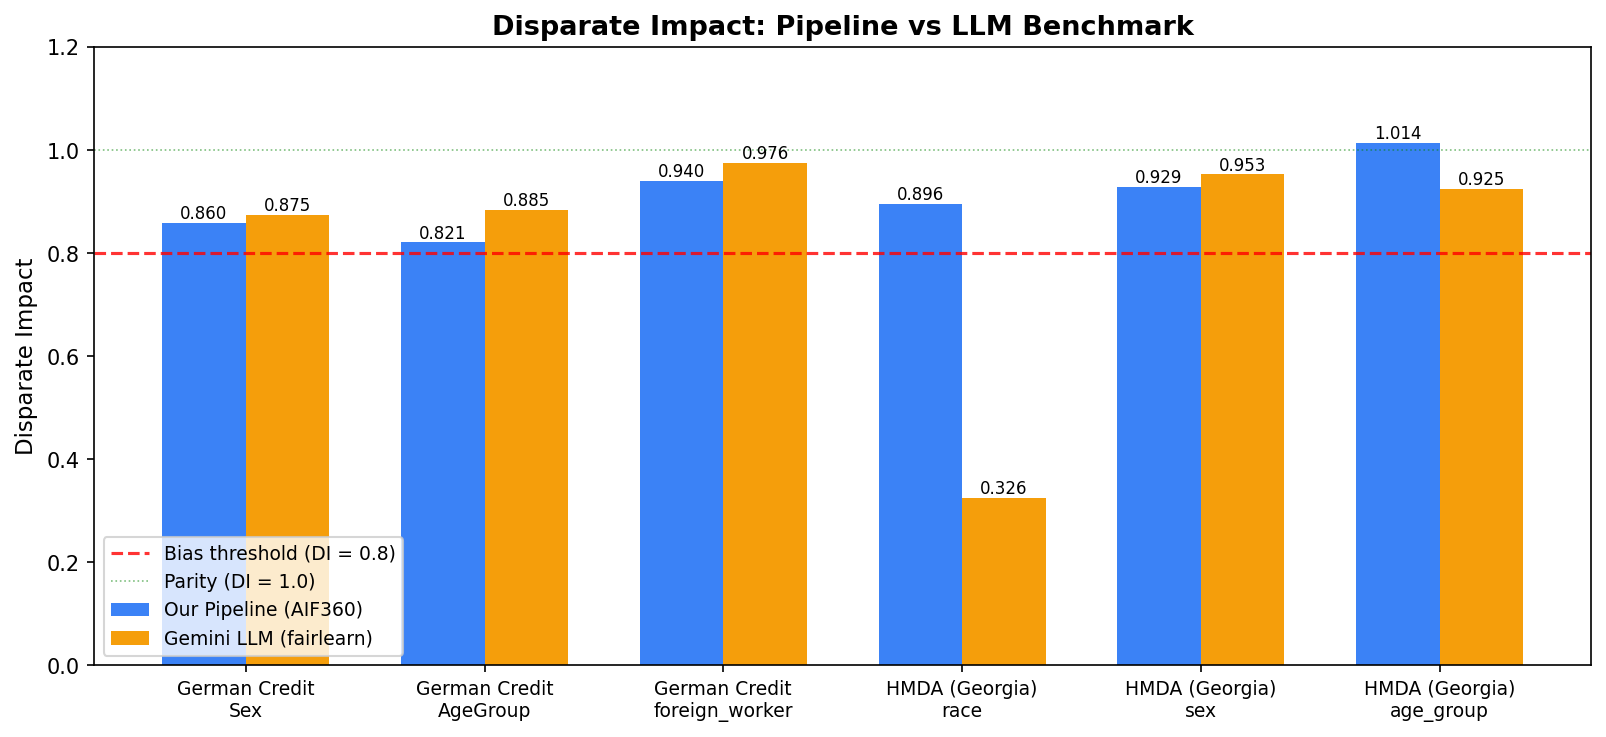
\includegraphics[width=\textwidth]{di_overview.png}
\caption{Disparate Impact overview across all datasets and attributes.}
\label{fig:di-overview}
\end{figure}

\begin{figure}[H]
\centering
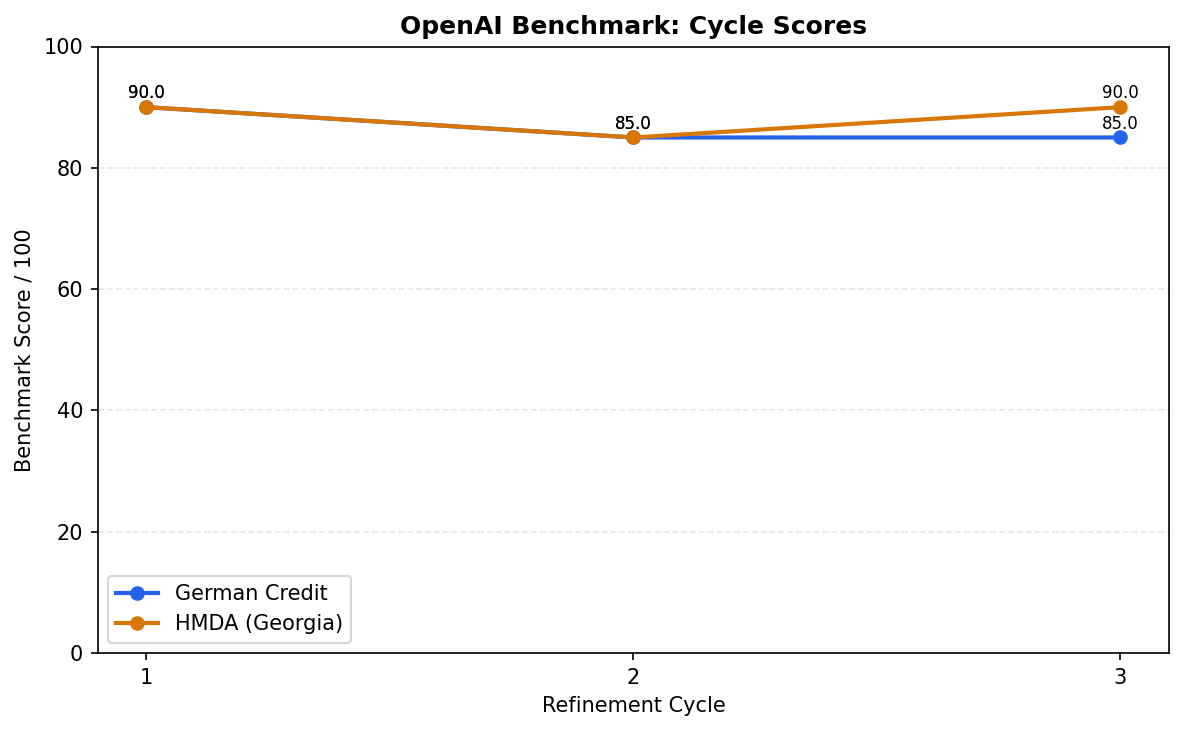
\includegraphics[width=0.85\textwidth]{openai_cycle_scores.png}
\caption{OpenAI benchmark cycle scores across fixed refinement cycles.}
\label{fig:openai-cycle-scores}
\end{figure}

\begin{figure}[H]
\centering
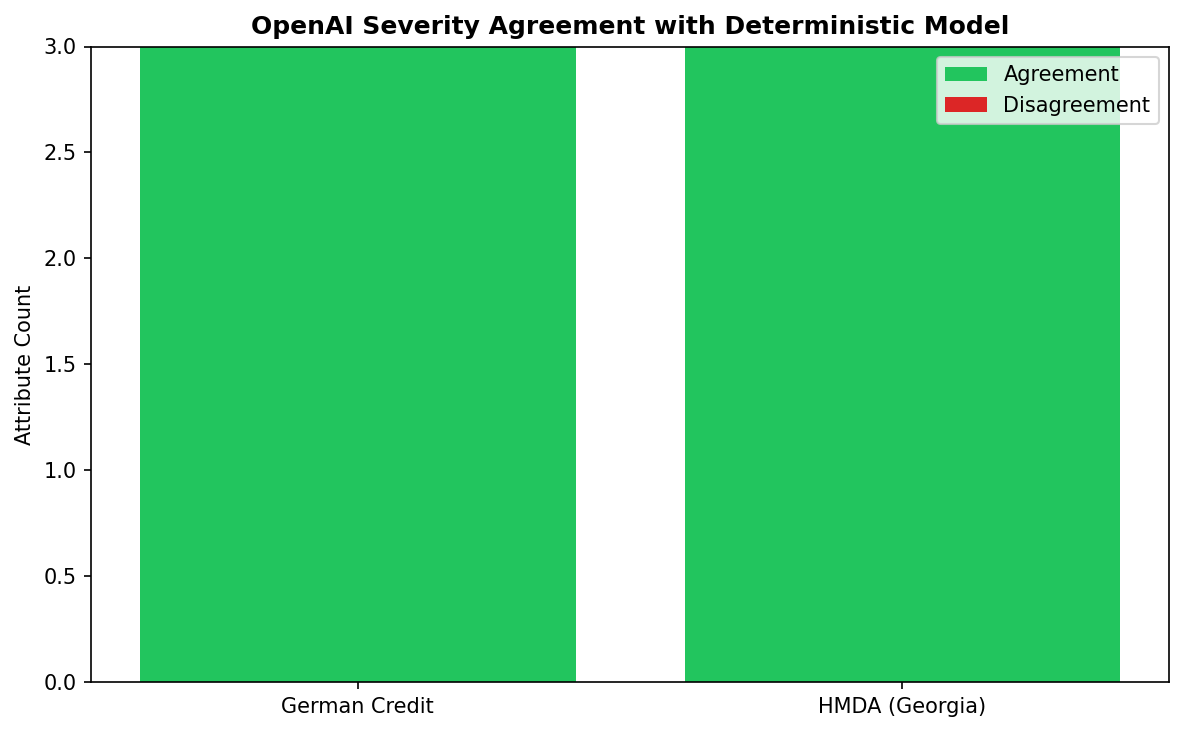
\includegraphics[width=0.9\textwidth]{openai_severity_agreement.png}
\caption{Severity agreement between deterministic baseline and OpenAI.}
\label{fig:severity}
\end{figure}

\subsection{Cost Analysis}

\begin{table}[H]
\centering
\caption{OpenAI benchmark cost breakdown (current artifact run).}
\label{tab:cost}
\begin{tabular}{lrrrr}
\toprule
\textbf{Dataset} & \textbf{Input Tokens} & \textbf{Output Tokens} & \textbf{Latency (s)} & \textbf{Est.\ Cost} \\
\midrule
German Credit & 3{,}862   & 2{,}182 & 29.7  & \$0.1259 \\
HMDA          & 4{,}032   & 1{,}666 & 14.2  & \$0.1070 \\
\midrule
\textbf{Total} & 7{,}894 & 3{,}848 & 43.9 & \textbf{\$0.2329} \\
\bottomrule
\end{tabular}
\end{table}

The benchmark remains inexpensive enough for artifact review, but cost and
latency depend on provider pricing, model selection, prompt length, and API
version.

\begin{figure}[H]
\centering
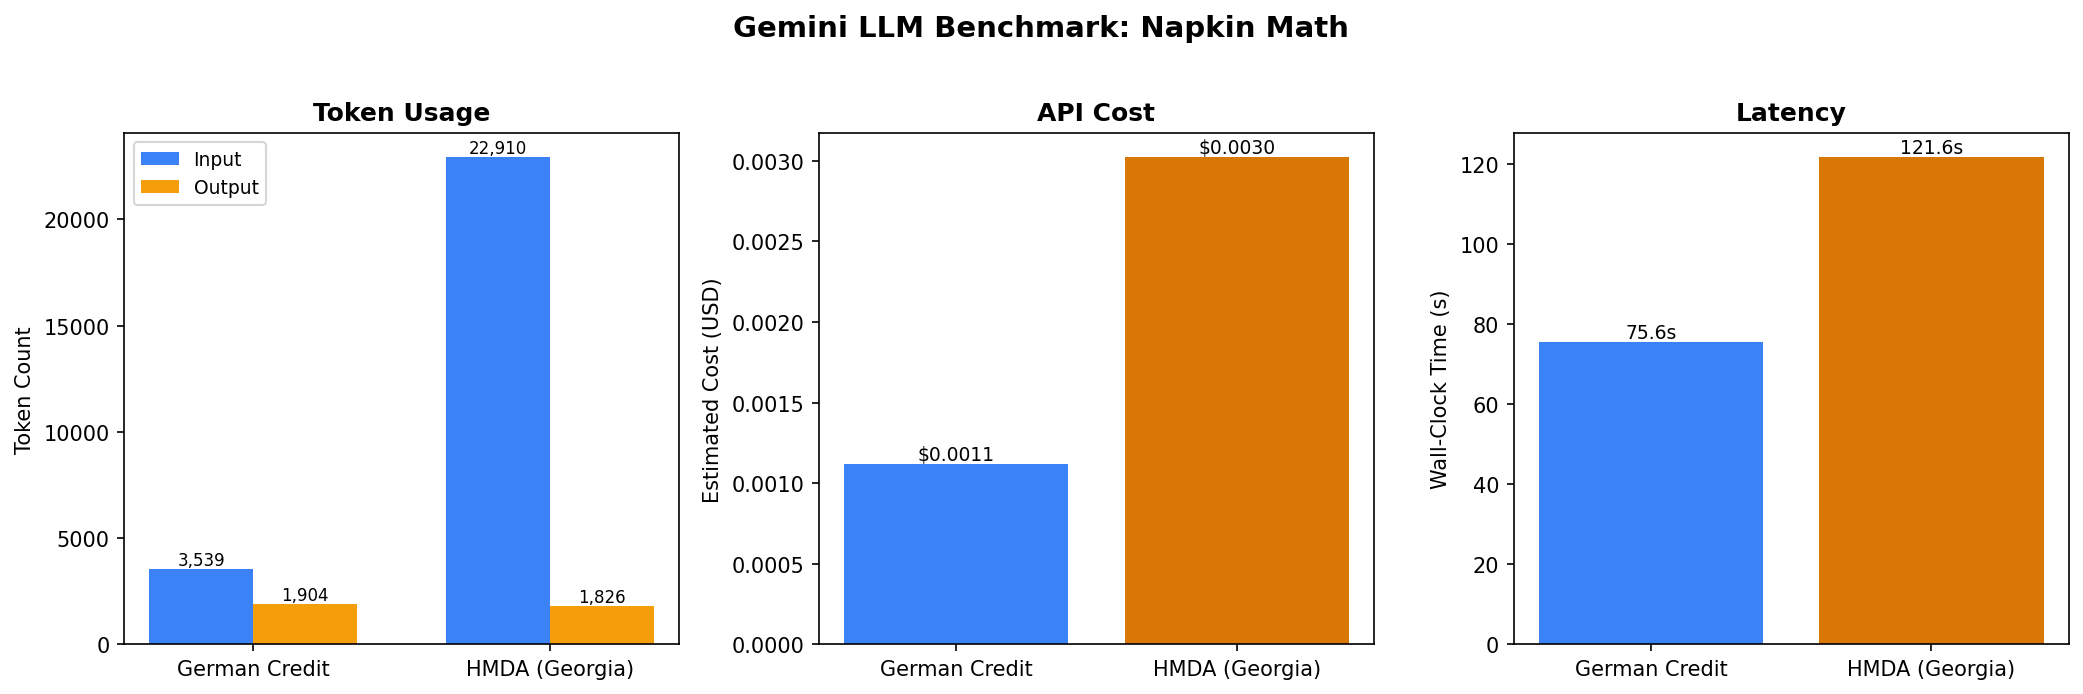
\includegraphics[width=\textwidth]{cost_summary.png}
\caption{Token usage, API cost, and latency per dataset.}
\label{fig:cost}
\end{figure}

% ===================================================================
\section{Discussion}

\subsection{Where Pipeline and OpenAI Agree}

OpenAI preserved the deterministic severity labels for all six
dataset-attribute pairs in the current artifact run. This is the desired
behavior under our protocol: the LLM should not create its own metric
baseline, but should translate the fixed metric evidence into clearer
remediation guidance. The strongest agreement appears for German Credit Sex
and AgeGroup and HMDA Race, where both the deterministic report and OpenAI
identify moderate disparities and recommend pre-processing, constrained
training, or post-processing interventions.

\subsection{Where the Benchmark Exposes Risk}

The main risk is not arithmetic disagreement, because arithmetic is owned by
the deterministic pipeline. The risk is \textbf{narrative overreach}: an LLM
can produce plausible causal language or detailed mitigation plans that
exceed the evidence available in the artifact. This is especially important
for small subgroups such as German Credit foreign-worker status and rare
HMDA race categories. The protocol therefore records context payloads,
baseline severities, prompt text, raw responses, and scoring outputs so that
reviewers can inspect whether LLM claims stay grounded in the provided
metric evidence.

Legacy Gemini runs illustrate a complementary failure mode: when an LLM is
asked to compute or choose metric baselines itself, small subgroup choices
can dominate the result and produce unstable severity labels. This motivates
the OpenAI-primary design used for the submission artifact.

\subsection{Strengths and Limitations}

\paragraph{Deterministic pipeline.}
Strengths: fully reproducible, transparent rule logic, specific AIF360
mitigation recommendations, statistical safeguards (minimum group size,
confidence warnings). Limitations: rigid rule structure cannot capture
novel bias patterns; qualitative explanations are templated.

\paragraph{LLM benchmark.}
Strengths: richer, more natural-language explanations; can identify
context-specific issues and convert metric tables into operational
recommendations. Limitations: possible narrative overreach; nondeterminism
across runs and API/model versions; sensitivity to prompt design; higher
latency and cost than deterministic Python; and dependence on Python context
for metric grounding.

\subsection{Value of Qualitative Analysis}

Raw fairness metrics alone are insufficient for actionable remediation.
A DI of 0.82 does not explain \emph{why} the model is biased or
\emph{what to do about it}. Our qualitative engine bridges this gap:
for AgeGroup, it identifies that (a) the Age feature is a strong proxy
($r{=}{-}0.84$), (b) ground-truth labels embed historical age
discrimination, and (c) specific AIF360 algorithms
(Reweighing, DisparateImpactRemover) can address these root causes.

% ===================================================================
\section{Conclusion and Future Work}

We presented a reproducible fairness-audit artifact for lending models that
combines deterministic quantitative metrics, deterministic qualitative
analysis, and an OpenAI benchmark for remediation-ready audit narratives. Key
findings:
\begin{itemize}[nosep]
  \item Both German Credit and HMDA exhibit \textsc{Moderate} bias on
        most protected attributes, driven by historical label disparities
        and proxy features.
  \item OpenAI agrees with deterministic severity labels in the current run
        when given fixed Python-computed metric context, but this should be
        interpreted as prompt- and model-version-specific rather than a
        universal guarantee.
  \item LLM auditing can improve remediation narrative quality, but requires
        explicit guardrails for metric grounding, subgroup-size uncertainty,
        reproducibility, and API/model versioning.
  \item The responsible-release materials---README, Docker/Make/CI scaffold,
        citation metadata, and data cards---are part of the artifact rather
        than ancillary documentation.
\end{itemize}

\paragraph{Future work.}
We plan to deepen our analysis within the finance and lending domain:
\begin{itemize}[nosep]
  \item \textbf{Additional lending datasets}: incorporate peer-to-peer
        lending and consumer credit bureau data to test generalizability.
  \item \textbf{Intersectional fairness}: analyze compound protected groups
        (e.g., race $\times$ sex) to detect bias invisible at single-attribute
        granularity.
  \item \textbf{End-to-end mitigation}: implement the recommended AIF360
        and fairlearn mitigations (Reweighing, ExponentiatedGradient,
        ThresholdOptimizer) and measure their impact on both accuracy and
        fairness.
  \item \textbf{Uncertainty-aware reporting}: add bootstrap confidence
        intervals or exact tests for small subgroups before escalating
        severity claims.
  \item \textbf{Longitudinal bias monitoring}: track fairness metric drift
        over time as data distributions shift, enabling early detection of
        emergent bias.
\end{itemize}

% ===================================================================
\begin{thebibliography}{9}

\bibitem{aif360}
R.~K.~E.~Bellamy et~al.,
``AI Fairness 360: An extensible toolkit for detecting and mitigating
algorithmic bias,''
\textit{IBM Journal of Research and Development}, vol.~63, no.~4/5, 2019.
\url{https://github.com/Trusted-AI/AIF360}

\bibitem{fairlearn}
S.~Bird et~al.,
``Fairlearn: A toolkit for assessing and improving fairness in AI,''
Microsoft Research, Tech.\ Rep., 2020.
\url{https://fairlearn.org}

\bibitem{german}
H.~Hofmann,
``Statlog (German Credit Data),''
UCI Machine Learning Repository, 1994.
\url{https://archive.ics.uci.edu/ml/datasets/statlog+(german+credit+data)}

\bibitem{hmda}
Consumer Financial Protection Bureau,
``HMDA Data Browser,''
\url{https://ffiec.cfpb.gov/data-browser/}

\bibitem{openai}
OpenAI,
``OpenAI API Documentation,''
\url{https://platform.openai.com/docs}

\end{thebibliography}

\end{document}
